\begin{figure}[ht]
\begin{center}
\begin{adjustbox}{width=0.7\textwidth}


\tikzset{every picture/.style={line width=0.75pt}} %set default line width to 0.75pt        

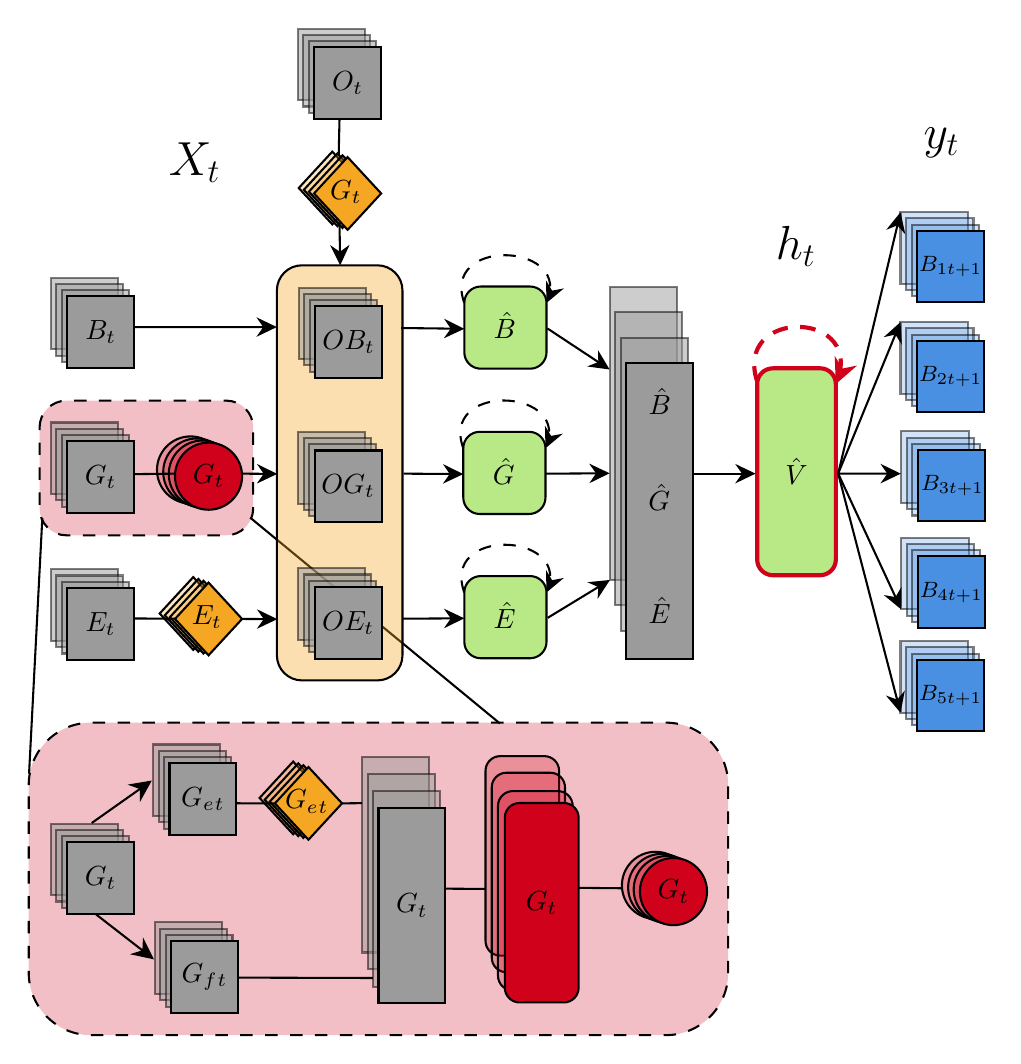
\begin{tikzpicture}[x=0.75pt,y=0.75pt,yscale=-1,xscale=1]
%uncomment if require: \path (0,532); %set diagram left start at 0, and has height of 532

%Rounded Rect [id:dp08035828151528335] 
\draw  [fill={rgb, 255:red, 208; green, 2; blue, 27 }  ,fill opacity=0.25 ][dash pattern={on 4.5pt off 4.5pt}] (101.33,385.5) .. controls (101.33,368.87) and (114.82,355.39) .. (131.45,355.39) -- (408.22,355.39) .. controls (424.85,355.39) and (438.33,368.87) .. (438.33,385.5) -- (438.33,475.85) .. controls (438.33,492.48) and (424.85,505.96) .. (408.22,505.96) -- (131.45,505.96) .. controls (114.82,505.96) and (101.33,492.48) .. (101.33,475.85) -- cycle ;
%Rounded Rect [id:dp022539755099525105] 
\draw  [color={rgb, 255:red, 0; green, 0; blue, 0 }  ,draw opacity=1 ][fill={rgb, 255:red, 208; green, 2; blue, 27 }  ,fill opacity=0.25 ][line width=0.75]  (321.41,378.62) .. controls (321.41,374.7) and (324.59,371.53) .. (328.5,371.53) -- (349.77,371.53) .. controls (353.68,371.53) and (356.86,374.7) .. (356.86,378.62) -- (356.86,460.54) .. controls (356.86,464.45) and (353.68,467.63) .. (349.77,467.63) -- (328.5,467.63) .. controls (324.59,467.63) and (321.41,464.45) .. (321.41,460.54) -- cycle ;
%Rounded Rect [id:dp773732764610876] 
\draw  [color={rgb, 255:red, 0; green, 0; blue, 0 }  ,draw opacity=1 ][fill={rgb, 255:red, 208; green, 2; blue, 27 }  ,fill opacity=0.25 ][line width=0.75]  (324.41,386.59) .. controls (324.41,382.69) and (327.58,379.53) .. (331.47,379.53) -- (352.65,379.53) .. controls (356.55,379.53) and (359.71,382.69) .. (359.71,386.59) -- (359.71,468.57) .. controls (359.71,472.47) and (356.55,475.63) .. (352.65,475.63) -- (331.47,475.63) .. controls (327.58,475.63) and (324.41,472.47) .. (324.41,468.57) -- cycle ;
%Rounded Rect [id:dp821346761617826] 
\draw  [color={rgb, 255:red, 0; green, 0; blue, 0 }  ,draw opacity=1 ][fill={rgb, 255:red, 208; green, 2; blue, 27 }  ,fill opacity=0.25 ][line width=0.75]  (327.41,395.56) .. controls (327.41,391.59) and (330.64,388.36) .. (334.62,388.36) -- (356.23,388.36) .. controls (360.2,388.36) and (363.43,391.59) .. (363.43,395.56) -- (363.43,477.26) .. controls (363.43,481.24) and (360.2,484.46) .. (356.23,484.46) -- (334.62,484.46) .. controls (330.64,484.46) and (327.41,481.24) .. (327.41,477.26) -- cycle ;
%Straight Lines [id:da8816584047486795] 
\draw    (208,256.6) -- (328.33,355.77) ;
%Straight Lines [id:da4915418231679166] 
\draw    (107.88,256.89) -- (101.5,379.93) ;
%Rounded Rect [id:dp8378752434652124] 
\draw  [fill={rgb, 255:red, 208; green, 2; blue, 27 }  ,fill opacity=0.25 ][dash pattern={on 4.5pt off 4.5pt}] (106.56,213.23) .. controls (106.56,206.07) and (112.37,200.25) .. (119.54,200.25) -- (196.49,200.25) .. controls (203.66,200.25) and (209.47,206.07) .. (209.47,213.23) -- (209.47,252.17) .. controls (209.47,259.33) and (203.66,265.14) .. (196.49,265.14) -- (119.54,265.14) .. controls (112.37,265.14) and (106.56,259.33) .. (106.56,252.17) -- cycle ;
%Shape: Circle [id:dp7319115465111494] 
\draw  [fill={rgb, 255:red, 208; green, 2; blue, 27 }  ,fill opacity=0.25 ] (163.13,233.65) .. controls (163.13,224.72) and (170.37,217.48) .. (179.3,217.48) .. controls (188.23,217.48) and (195.47,224.72) .. (195.47,233.65) .. controls (195.47,242.58) and (188.23,249.82) .. (179.3,249.82) .. controls (170.37,249.82) and (163.13,242.58) .. (163.13,233.65) -- cycle ;
%Shape: Circle [id:dp20640118029319288] 
\draw  [fill={rgb, 255:red, 208; green, 2; blue, 27 }  ,fill opacity=0.25 ] (166.13,234.65) .. controls (166.13,225.72) and (173.37,218.48) .. (182.3,218.48) .. controls (191.23,218.48) and (198.47,225.72) .. (198.47,234.65) .. controls (198.47,243.58) and (191.23,250.82) .. (182.3,250.82) .. controls (173.37,250.82) and (166.13,243.58) .. (166.13,234.65) -- cycle ;
%Shape: Circle [id:dp9035374173552181] 
\draw  [fill={rgb, 255:red, 208; green, 2; blue, 27 }  ,fill opacity=0.25 ] (168.8,235.65) .. controls (168.8,226.72) and (176.04,219.48) .. (184.97,219.48) .. controls (193.9,219.48) and (201.13,226.72) .. (201.13,235.65) .. controls (201.13,244.58) and (193.9,251.82) .. (184.97,251.82) .. controls (176.04,251.82) and (168.8,244.58) .. (168.8,235.65) -- cycle ;
%Shape: Circle [id:dp2977025290564278] 
\draw  [fill={rgb, 255:red, 208; green, 2; blue, 27 }  ,fill opacity=1 ] (171.8,236.65) .. controls (171.8,227.72) and (179.04,220.48) .. (187.97,220.48) .. controls (196.9,220.48) and (204.13,227.72) .. (204.13,236.65) .. controls (204.13,245.58) and (196.9,252.82) .. (187.97,252.82) .. controls (179.04,252.82) and (171.8,245.58) .. (171.8,236.65) -- cycle ;

%Rounded Rect [id:dp15650356150345013] 
\draw  [fill={rgb, 255:red, 245; green, 166; blue, 35 }  ,fill opacity=0.36 ] (220.9,147.15) .. controls (220.9,140.47) and (226.32,135.05) .. (233,135.05) -- (269.3,135.05) .. controls (275.98,135.05) and (281.4,140.47) .. (281.4,147.15) -- (281.4,322.95) .. controls (281.4,329.63) and (275.98,335.05) .. (269.3,335.05) -- (233,335.05) .. controls (226.32,335.05) and (220.9,329.63) .. (220.9,322.95) -- cycle ;
%Straight Lines [id:da409284418173784] 
\draw    (251.06,114.76) -- (251.35,132.05) ;
\draw [shift={(251.4,135.05)}, rotate = 269.03] [fill={rgb, 255:red, 0; green, 0; blue, 0 }  ][line width=0.08]  [draw opacity=0] (9.82,-4.72) -- (0,0) -- (9.82,4.72) -- (6.52,0) -- cycle    ;
%Shape: Rectangle [id:dp7034345660290355] 
\draw  [color={rgb, 255:red, 0; green, 0; blue, 0 }  ,draw opacity=0.5 ][fill={rgb, 255:red, 155; green, 155; blue, 155 }  ,fill opacity=0.5 ] (112.01,281.53) -- (144.26,281.53) -- (144.26,316.05) -- (112.01,316.05) -- cycle ;
%Shape: Rectangle [id:dp22118233628007533] 
\draw  [color={rgb, 255:red, 0; green, 0; blue, 0 }  ,draw opacity=0.5 ][fill={rgb, 255:red, 155; green, 155; blue, 155 }  ,fill opacity=0.5 ] (114.63,284.51) -- (146.88,284.51) -- (146.88,319.03) -- (114.63,319.03) -- cycle ;
%Shape: Rectangle [id:dp24867768000931467] 
\draw  [color={rgb, 255:red, 0; green, 0; blue, 0 }  ,draw opacity=0.5 ][fill={rgb, 255:red, 155; green, 155; blue, 155 }  ,fill opacity=0.5 ] (117.27,287.56) -- (149.53,287.56) -- (149.53,322.08) -- (117.27,322.08) -- cycle ;
%Shape: Rectangle [id:dp124905579804508] 
\draw  [fill={rgb, 255:red, 155; green, 155; blue, 155 }  ,fill opacity=1 ] (119.86,290.5) -- (152.11,290.5) -- (152.11,325.02) -- (119.86,325.02) -- cycle ;
%Straight Lines [id:da8537240673366849] 
\draw    (251.06,64.86) -- (250.67,82.43) ;
%Rounded Rect [id:dp9724403504665806] 
\draw  [color={rgb, 255:red, 208; green, 2; blue, 27 }  ,draw opacity=1 ][fill={rgb, 255:red, 184; green, 233; blue, 134 }  ,fill opacity=1 ][line width=1.5]  (452.3,192.25) .. controls (452.3,188.06) and (455.7,184.67) .. (459.88,184.67) -- (482.62,184.67) .. controls (486.81,184.67) and (490.2,188.06) .. (490.2,192.25) -- (490.2,276.79) .. controls (490.2,280.97) and (486.81,284.37) .. (482.62,284.37) -- (459.88,284.37) .. controls (455.7,284.37) and (452.3,280.97) .. (452.3,276.79) -- cycle ;
%Curve Lines [id:da6973720397061056] 
\draw [color={rgb, 255:red, 208; green, 2; blue, 27 }  ,draw opacity=1 ][line width=1.5]  [dash pattern={on 5.63pt off 4.5pt}]  (452.3,191.02) .. controls (440.95,156.4) and (501.2,156.33) .. (491.53,188.61) ;
\draw [shift={(490.2,192.25)}, rotate = 293.32] [fill={rgb, 255:red, 208; green, 2; blue, 27 }  ,fill opacity=1 ][line width=0.08]  [draw opacity=0] (12.23,-5.88) -- (0,0) -- (12.23,5.88) -- (8.12,0) -- cycle    ;
%Shape: Rectangle [id:dp1958055080757597] 
\draw  [color={rgb, 255:red, 0; green, 0; blue, 0 }  ,draw opacity=0.5 ][fill={rgb, 255:red, 74; green, 144; blue, 226 }  ,fill opacity=0.25 ] (521.36,162.39) -- (553.87,162.39) -- (553.87,196.9) -- (521.36,196.9) -- cycle ;
%Shape: Rectangle [id:dp20825701586292622] 
\draw  [color={rgb, 255:red, 0; green, 0; blue, 0 }  ,draw opacity=0.5 ][fill={rgb, 255:red, 74; green, 144; blue, 226 }  ,fill opacity=0.25 ] (524,165.37) -- (556.51,165.37) -- (556.51,199.88) -- (524,199.88) -- cycle ;
%Shape: Rectangle [id:dp6709034910590727] 
\draw  [color={rgb, 255:red, 0; green, 0; blue, 0 }  ,draw opacity=0.5 ][fill={rgb, 255:red, 74; green, 144; blue, 226 }  ,fill opacity=0.25 ] (526.67,168.42) -- (559.17,168.42) -- (559.17,202.93) -- (526.67,202.93) -- cycle ;
%Shape: Rectangle [id:dp943426610209301] 
\draw  [fill={rgb, 255:red, 74; green, 144; blue, 226 }  ,fill opacity=1 ] (529.28,171.36) -- (561.78,171.36) -- (561.78,205.87) -- (529.28,205.87) -- cycle ;
%Shape: Rectangle [id:dp9270730461824767] 
\draw  [color={rgb, 255:red, 0; green, 0; blue, 0 }  ,draw opacity=0.5 ][fill={rgb, 255:red, 74; green, 144; blue, 226 }  ,fill opacity=0.25 ] (521.69,215.06) -- (554.2,215.06) -- (554.2,249.56) -- (521.69,249.56) -- cycle ;
%Shape: Rectangle [id:dp9671567967621458] 
\draw  [color={rgb, 255:red, 0; green, 0; blue, 0 }  ,draw opacity=0.5 ][fill={rgb, 255:red, 74; green, 144; blue, 226 }  ,fill opacity=0.25 ] (524.33,218.04) -- (556.84,218.04) -- (556.84,252.54) -- (524.33,252.54) -- cycle ;
%Shape: Rectangle [id:dp6567850092606636] 
\draw  [color={rgb, 255:red, 0; green, 0; blue, 0 }  ,draw opacity=0.5 ][fill={rgb, 255:red, 74; green, 144; blue, 226 }  ,fill opacity=0.25 ] (527,221.09) -- (559.5,221.09) -- (559.5,255.6) -- (527,255.6) -- cycle ;
%Shape: Rectangle [id:dp9307909660529495] 
\draw  [fill={rgb, 255:red, 74; green, 144; blue, 226 }  ,fill opacity=1 ] (529.62,224.02) -- (561.84,224.02) -- (561.84,258.22) -- (529.62,258.22) -- cycle ;
%Shape: Rectangle [id:dp2956426995252315] 
\draw  [color={rgb, 255:red, 0; green, 0; blue, 0 }  ,draw opacity=0.5 ][fill={rgb, 255:red, 74; green, 144; blue, 226 }  ,fill opacity=0.25 ] (521.36,316.11) -- (553.87,316.11) -- (553.87,350.62) -- (521.36,350.62) -- cycle ;
%Shape: Rectangle [id:dp9676718309145981] 
\draw  [color={rgb, 255:red, 0; green, 0; blue, 0 }  ,draw opacity=0.5 ][fill={rgb, 255:red, 74; green, 144; blue, 226 }  ,fill opacity=0.25 ] (524,319.09) -- (556.51,319.09) -- (556.51,353.6) -- (524,353.6) -- cycle ;
%Shape: Rectangle [id:dp3802447939611997] 
\draw  [color={rgb, 255:red, 0; green, 0; blue, 0 }  ,draw opacity=0.5 ][fill={rgb, 255:red, 74; green, 144; blue, 226 }  ,fill opacity=0.25 ] (526.67,322.14) -- (559.17,322.14) -- (559.17,356.65) -- (526.67,356.65) -- cycle ;
%Shape: Rectangle [id:dp2655409211543931] 
\draw  [fill={rgb, 255:red, 74; green, 144; blue, 226 }  ,fill opacity=1 ] (529.28,325.08) -- (561.78,325.08) -- (561.78,359.59) -- (529.28,359.59) -- cycle ;
%Shape: Rectangle [id:dp4040153422296009] 
\draw  [color={rgb, 255:red, 0; green, 0; blue, 0 }  ,draw opacity=0.5 ][fill={rgb, 255:red, 74; green, 144; blue, 226 }  ,fill opacity=0.25 ] (521.69,266.32) -- (554.2,266.32) -- (554.2,300.83) -- (521.69,300.83) -- cycle ;
%Shape: Rectangle [id:dp7066102537923638] 
\draw  [color={rgb, 255:red, 0; green, 0; blue, 0 }  ,draw opacity=0.5 ][fill={rgb, 255:red, 74; green, 144; blue, 226 }  ,fill opacity=0.25 ] (524.33,269.3) -- (556.84,269.3) -- (556.84,303.81) -- (524.33,303.81) -- cycle ;
%Shape: Rectangle [id:dp46050637304135866] 
\draw  [color={rgb, 255:red, 0; green, 0; blue, 0 }  ,draw opacity=0.5 ][fill={rgb, 255:red, 74; green, 144; blue, 226 }  ,fill opacity=0.25 ] (527,272.35) -- (559.5,272.35) -- (559.5,306.86) -- (527,306.86) -- cycle ;
%Shape: Rectangle [id:dp2033829273595421] 
\draw  [fill={rgb, 255:red, 74; green, 144; blue, 226 }  ,fill opacity=1 ] (529.61,275.29) -- (562.11,275.29) -- (562.11,309.8) -- (529.61,309.8) -- cycle ;
%Shape: Rectangle [id:dp19424752965877823] 
\draw  [color={rgb, 255:red, 0; green, 0; blue, 0 }  ,draw opacity=0.5 ][fill={rgb, 255:red, 74; green, 144; blue, 226 }  ,fill opacity=0.25 ] (521.36,109.48) -- (553.87,109.48) -- (553.87,143.98) -- (521.36,143.98) -- cycle ;
%Shape: Rectangle [id:dp6987771152166413] 
\draw  [color={rgb, 255:red, 0; green, 0; blue, 0 }  ,draw opacity=0.5 ][fill={rgb, 255:red, 74; green, 144; blue, 226 }  ,fill opacity=0.25 ] (524,112.46) -- (556.51,112.46) -- (556.51,146.96) -- (524,146.96) -- cycle ;
%Shape: Rectangle [id:dp12765942569283661] 
\draw  [color={rgb, 255:red, 0; green, 0; blue, 0 }  ,draw opacity=0.5 ][fill={rgb, 255:red, 74; green, 144; blue, 226 }  ,fill opacity=0.25 ] (526.67,115.51) -- (559.17,115.51) -- (559.17,150.01) -- (526.67,150.01) -- cycle ;
%Shape: Rectangle [id:dp16248810139444148] 
\draw  [fill={rgb, 255:red, 74; green, 144; blue, 226 }  ,fill opacity=1 ] (529.28,118.44) -- (561.78,118.44) -- (561.78,152.95) -- (529.28,152.95) -- cycle ;
%Shape: Rectangle [id:dp7988673729176894] 
\draw  [color={rgb, 255:red, 0; green, 0; blue, 0 }  ,draw opacity=0.5 ][fill={rgb, 255:red, 155; green, 155; blue, 155 }  ,fill opacity=0.5 ] (112.01,210.77) -- (144.26,210.77) -- (144.26,245.29) -- (112.01,245.29) -- cycle ;
%Shape: Rectangle [id:dp9623129937085917] 
\draw  [color={rgb, 255:red, 0; green, 0; blue, 0 }  ,draw opacity=0.5 ][fill={rgb, 255:red, 155; green, 155; blue, 155 }  ,fill opacity=0.5 ] (114.63,213.75) -- (146.88,213.75) -- (146.88,248.27) -- (114.63,248.27) -- cycle ;
%Shape: Rectangle [id:dp429379441325212] 
\draw  [color={rgb, 255:red, 0; green, 0; blue, 0 }  ,draw opacity=0.5 ][fill={rgb, 255:red, 155; green, 155; blue, 155 }  ,fill opacity=0.5 ] (117.27,216.8) -- (149.53,216.8) -- (149.53,251.32) -- (117.27,251.32) -- cycle ;
%Shape: Rectangle [id:dp9493890675957639] 
\draw  [fill={rgb, 255:red, 155; green, 155; blue, 155 }  ,fill opacity=1 ] (119.86,219.74) -- (152.11,219.74) -- (152.11,254.26) -- (119.86,254.26) -- cycle ;
%Straight Lines [id:da0399560958706785] 
\draw [fill={rgb, 255:red, 155; green, 155; blue, 155 }  ,fill opacity=1 ]   (151.09,164.83) -- (217.85,164.8) ;
\draw [shift={(220.85,164.8)}, rotate = 179.98] [fill={rgb, 255:red, 0; green, 0; blue, 0 }  ][line width=0.08]  [draw opacity=0] (9.82,-4.72) -- (0,0) -- (9.82,4.72) -- (6.52,0) -- cycle    ;
%Shape: Rectangle [id:dp3393145890474042] 
\draw  [color={rgb, 255:red, 0; green, 0; blue, 0 }  ,draw opacity=0.5 ][fill={rgb, 255:red, 155; green, 155; blue, 155 }  ,fill opacity=0.5 ] (112.01,141.06) -- (144.26,141.06) -- (144.26,175.57) -- (112.01,175.57) -- cycle ;
%Shape: Rectangle [id:dp27631704382885136] 
\draw  [color={rgb, 255:red, 0; green, 0; blue, 0 }  ,draw opacity=0.5 ][fill={rgb, 255:red, 155; green, 155; blue, 155 }  ,fill opacity=0.5 ] (114.63,144.04) -- (146.88,144.04) -- (146.88,178.55) -- (114.63,178.55) -- cycle ;
%Shape: Rectangle [id:dp8553441662393909] 
\draw  [color={rgb, 255:red, 0; green, 0; blue, 0 }  ,draw opacity=0.5 ][fill={rgb, 255:red, 155; green, 155; blue, 155 }  ,fill opacity=0.5 ] (117.27,147.09) -- (149.53,147.09) -- (149.53,181.61) -- (117.27,181.61) -- cycle ;
%Shape: Rectangle [id:dp4571491350911555] 
\draw  [fill={rgb, 255:red, 155; green, 155; blue, 155 }  ,fill opacity=1 ] (119.86,150.03) -- (152.11,150.03) -- (152.11,184.54) -- (119.86,184.54) -- cycle ;
%Straight Lines [id:da3169233008507637] 
\draw    (152.46,235.66) -- (171.8,235.43) ;
%Shape: Diamond [id:dp08100159339963764] 
\draw  [fill={rgb, 255:red, 245; green, 166; blue, 35 }  ,fill opacity=0.25 ] (180.6,285.28) -- (196.77,302.81) -- (180.6,320.33) -- (164.43,302.81) -- cycle ;
%Shape: Diamond [id:dp6545409040088919] 
\draw  [fill={rgb, 255:red, 245; green, 166; blue, 35 }  ,fill opacity=0.25 ] (183.05,286.16) -- (199.22,303.68) -- (183.05,321.2) -- (166.89,303.68) -- cycle ;
%Shape: Diamond [id:dp22008618792927115] 
\draw  [fill={rgb, 255:red, 245; green, 166; blue, 35 }  ,fill opacity=0.25 ] (185.51,287.04) -- (201.68,304.56) -- (185.51,322.08) -- (169.34,304.56) -- cycle ;
%Shape: Diamond [id:dp6216162169932065] 
\draw  [fill={rgb, 255:red, 245; green, 166; blue, 35 }  ,fill opacity=1 ] (187.97,287.91) -- (204.13,305.43) -- (187.97,322.96) -- (171.8,305.43) -- cycle ;
%Straight Lines [id:da6348314705630924] 
\draw    (204.13,305.43) -- (218.07,305.51) ;
\draw [shift={(221.07,305.53)}, rotate = 180.32] [fill={rgb, 255:red, 0; green, 0; blue, 0 }  ][line width=0.08]  [draw opacity=0] (9.82,-4.72) -- (0,0) -- (9.82,4.72) -- (6.52,0) -- cycle    ;
%Straight Lines [id:da29443986089740126] 
\draw    (151.89,305.2) -- (171.89,305.31) ;
%Straight Lines [id:da7037674707293678] 
\draw [fill={rgb, 255:red, 155; green, 155; blue, 155 }  ,fill opacity=1 ]   (280.77,165.26) -- (308.2,165.6) ;
\draw [shift={(311.2,165.63)}, rotate = 180.71] [fill={rgb, 255:red, 0; green, 0; blue, 0 }  ][line width=0.08]  [draw opacity=0] (9.82,-4.72) -- (0,0) -- (9.82,4.72) -- (6.52,0) -- cycle    ;
%Rounded Rect [id:dp05798817292021641] 
\draw  [color={rgb, 255:red, 0; green, 0; blue, 0 }  ,draw opacity=1 ][fill={rgb, 255:red, 184; green, 233; blue, 134 }  ,fill opacity=1 ][line width=0.75]  (311.2,153.19) .. controls (311.2,148.81) and (314.75,145.27) .. (319.12,145.27) -- (342.88,145.27) .. controls (347.25,145.27) and (350.8,148.81) .. (350.8,153.19) -- (350.8,176.95) .. controls (350.8,181.32) and (347.25,184.87) .. (342.88,184.87) -- (319.12,184.87) .. controls (314.75,184.87) and (311.2,181.32) .. (311.2,176.95) -- cycle ;
%Curve Lines [id:da04021743223527896] 
\draw [color={rgb, 255:red, 0; green, 0; blue, 0 }  ,draw opacity=1 ][line width=0.75]  [dash pattern={on 4.5pt off 4.5pt}]  (311.2,153.19) .. controls (299.92,122.06) and (360.25,123.81) .. (351.79,150.63) ;
\draw [shift={(350.8,153.19)}, rotate = 294.37] [fill={rgb, 255:red, 0; green, 0; blue, 0 }  ,fill opacity=1 ][line width=0.08]  [draw opacity=0] (9.82,-4.72) -- (0,0) -- (9.82,4.72) -- (6.52,0) -- cycle    ;
%Straight Lines [id:da04725287763752273] 
\draw [fill={rgb, 255:red, 155; green, 155; blue, 155 }  ,fill opacity=1 ]   (351.2,165.45) -- (378.7,183.6) ;
\draw [shift={(381.2,185.25)}, rotate = 213.42] [fill={rgb, 255:red, 0; green, 0; blue, 0 }  ][line width=0.08]  [draw opacity=0] (9.82,-4.72) -- (0,0) -- (9.82,4.72) -- (6.52,0) -- cycle    ;
%Straight Lines [id:da6945773359077246] 
\draw    (204.13,235.43) -- (218.07,235.54) ;
\draw [shift={(221.07,235.56)}, rotate = 180.44] [fill={rgb, 255:red, 0; green, 0; blue, 0 }  ][line width=0.08]  [draw opacity=0] (9.82,-4.72) -- (0,0) -- (9.82,4.72) -- (6.52,0) -- cycle    ;
%Straight Lines [id:da6273046628189572] 
\draw [fill={rgb, 255:red, 155; green, 155; blue, 155 }  ,fill opacity=1 ]   (281.91,235.43) -- (307.7,235.61) ;
\draw [shift={(310.7,235.63)}, rotate = 180.41] [fill={rgb, 255:red, 0; green, 0; blue, 0 }  ][line width=0.08]  [draw opacity=0] (9.82,-4.72) -- (0,0) -- (9.82,4.72) -- (6.52,0) -- cycle    ;
%Rounded Rect [id:dp7958241287205053] 
\draw  [color={rgb, 255:red, 0; green, 0; blue, 0 }  ,draw opacity=1 ][fill={rgb, 255:red, 184; green, 233; blue, 134 }  ,fill opacity=1 ][line width=0.75]  (310.7,223.19) .. controls (310.7,218.81) and (314.25,215.27) .. (318.62,215.27) -- (342.38,215.27) .. controls (346.75,215.27) and (350.3,218.81) .. (350.3,223.19) -- (350.3,246.95) .. controls (350.3,251.32) and (346.75,254.87) .. (342.38,254.87) -- (318.62,254.87) .. controls (314.25,254.87) and (310.7,251.32) .. (310.7,246.95) -- cycle ;
%Curve Lines [id:da19079237969225638] 
\draw [color={rgb, 255:red, 0; green, 0; blue, 0 }  ,draw opacity=1 ][line width=0.75]  [dash pattern={on 4.5pt off 4.5pt}]  (310.7,223.19) .. controls (299.42,192.06) and (359.75,193.81) .. (351.29,220.63) ;
\draw [shift={(350.3,223.19)}, rotate = 294.37] [fill={rgb, 255:red, 0; green, 0; blue, 0 }  ,fill opacity=1 ][line width=0.08]  [draw opacity=0] (9.82,-4.72) -- (0,0) -- (9.82,4.72) -- (6.52,0) -- cycle    ;
%Straight Lines [id:da5724582303552335] 
\draw [fill={rgb, 255:red, 155; green, 155; blue, 155 }  ,fill opacity=1 ]   (281.63,305.31) -- (308.2,305.15) ;
\draw [shift={(311.2,305.13)}, rotate = 179.65] [fill={rgb, 255:red, 0; green, 0; blue, 0 }  ][line width=0.08]  [draw opacity=0] (9.82,-4.72) -- (0,0) -- (9.82,4.72) -- (6.52,0) -- cycle    ;
%Rounded Rect [id:dp6456487678445413] 
\draw  [color={rgb, 255:red, 0; green, 0; blue, 0 }  ,draw opacity=1 ][fill={rgb, 255:red, 184; green, 233; blue, 134 }  ,fill opacity=1 ][line width=0.75]  (311.2,292.69) .. controls (311.2,288.31) and (314.75,284.77) .. (319.12,284.77) -- (342.88,284.77) .. controls (347.25,284.77) and (350.8,288.31) .. (350.8,292.69) -- (350.8,316.45) .. controls (350.8,320.82) and (347.25,324.37) .. (342.88,324.37) -- (319.12,324.37) .. controls (314.75,324.37) and (311.2,320.82) .. (311.2,316.45) -- cycle ;
%Curve Lines [id:da6374705672660576] 
\draw [color={rgb, 255:red, 0; green, 0; blue, 0 }  ,draw opacity=1 ][line width=0.75]  [dash pattern={on 4.5pt off 4.5pt}]  (311.2,292.69) .. controls (299.92,261.56) and (360.25,263.31) .. (351.79,290.13) ;
\draw [shift={(350.8,292.69)}, rotate = 294.37] [fill={rgb, 255:red, 0; green, 0; blue, 0 }  ,fill opacity=1 ][line width=0.08]  [draw opacity=0] (9.82,-4.72) -- (0,0) -- (9.82,4.72) -- (6.52,0) -- cycle    ;
%Shape: Rectangle [id:dp53907172122875] 
\draw  [color={rgb, 255:red, 0; green, 0; blue, 0 }  ,draw opacity=0.5 ][fill={rgb, 255:red, 155; green, 155; blue, 155 }  ,fill opacity=0.5 ] (231.01,21.06) -- (263.26,21.06) -- (263.26,55.57) -- (231.01,55.57) -- cycle ;
%Shape: Rectangle [id:dp009192212091793661] 
\draw  [color={rgb, 255:red, 0; green, 0; blue, 0 }  ,draw opacity=0.5 ][fill={rgb, 255:red, 155; green, 155; blue, 155 }  ,fill opacity=0.5 ] (233.63,24.04) -- (265.88,24.04) -- (265.88,58.55) -- (233.63,58.55) -- cycle ;
%Shape: Rectangle [id:dp10982806096562447] 
\draw  [color={rgb, 255:red, 0; green, 0; blue, 0 }  ,draw opacity=0.5 ][fill={rgb, 255:red, 155; green, 155; blue, 155 }  ,fill opacity=0.5 ] (236.27,27.09) -- (268.53,27.09) -- (268.53,61.61) -- (236.27,61.61) -- cycle ;
%Shape: Rectangle [id:dp024787601372134982] 
\draw  [fill={rgb, 255:red, 155; green, 155; blue, 155 }  ,fill opacity=1 ] (238.86,30.03) -- (271.11,30.03) -- (271.11,64.54) -- (238.86,64.54) -- cycle ;
%Shape: Rectangle [id:dp9022114030928725] 
\draw  [color={rgb, 255:red, 0; green, 0; blue, 0 }  ,draw opacity=0.5 ][fill={rgb, 255:red, 155; green, 155; blue, 155 }  ,fill opacity=0.5 ] (381.34,145.45) -- (413.6,145.45) -- (413.6,286.66) -- (381.34,286.66) -- cycle ;
%Shape: Rectangle [id:dp9877830883323443] 
\draw  [color={rgb, 255:red, 0; green, 0; blue, 0 }  ,draw opacity=0.5 ][fill={rgb, 255:red, 155; green, 155; blue, 155 }  ,fill opacity=0.5 ] (383.96,157.64) -- (416.22,157.64) -- (416.22,298.84) -- (383.96,298.84) -- cycle ;
%Shape: Rectangle [id:dp8814167498359042] 
\draw  [color={rgb, 255:red, 0; green, 0; blue, 0 }  ,draw opacity=0.5 ][fill={rgb, 255:red, 155; green, 155; blue, 155 }  ,fill opacity=0.5 ] (386.61,170.13) -- (418.86,170.13) -- (418.86,311.34) -- (386.61,311.34) -- cycle ;
%Shape: Rectangle [id:dp5289911737134959] 
\draw  [fill={rgb, 255:red, 155; green, 155; blue, 155 }  ,fill opacity=1 ] (389.19,182.14) -- (421.45,182.14) -- (421.45,324.53) -- (389.19,324.53) -- cycle ;
%Shape: Rectangle [id:dp8149328215662492] 
\draw  [color={rgb, 255:red, 0; green, 0; blue, 0 }  ,draw opacity=0.5 ][fill={rgb, 255:red, 155; green, 155; blue, 155 }  ,fill opacity=0.5 ] (231.51,145.77) -- (263.76,145.77) -- (263.76,180.29) -- (231.51,180.29) -- cycle ;
%Shape: Rectangle [id:dp45921305478843055] 
\draw  [color={rgb, 255:red, 0; green, 0; blue, 0 }  ,draw opacity=0.5 ][fill={rgb, 255:red, 155; green, 155; blue, 155 }  ,fill opacity=0.5 ] (234.13,148.75) -- (266.38,148.75) -- (266.38,183.27) -- (234.13,183.27) -- cycle ;
%Shape: Rectangle [id:dp6228279530655318] 
\draw  [color={rgb, 255:red, 0; green, 0; blue, 0 }  ,draw opacity=0.5 ][fill={rgb, 255:red, 155; green, 155; blue, 155 }  ,fill opacity=0.5 ] (236.77,151.8) -- (269.03,151.8) -- (269.03,186.32) -- (236.77,186.32) -- cycle ;
%Shape: Rectangle [id:dp3598797805540589] 
\draw  [fill={rgb, 255:red, 155; green, 155; blue, 155 }  ,fill opacity=1 ] (239.36,154.74) -- (271.61,154.74) -- (271.61,189.26) -- (239.36,189.26) -- cycle ;
%Shape: Rectangle [id:dp9661891091990619] 
\draw  [color={rgb, 255:red, 0; green, 0; blue, 0 }  ,draw opacity=0.5 ][fill={rgb, 255:red, 155; green, 155; blue, 155 }  ,fill opacity=0.5 ] (231.26,215.32) -- (263.51,215.32) -- (263.51,249.84) -- (231.26,249.84) -- cycle ;
%Shape: Rectangle [id:dp690231151268716] 
\draw  [color={rgb, 255:red, 0; green, 0; blue, 0 }  ,draw opacity=0.5 ][fill={rgb, 255:red, 155; green, 155; blue, 155 }  ,fill opacity=0.5 ] (233.88,218.3) -- (266.13,218.3) -- (266.13,252.82) -- (233.88,252.82) -- cycle ;
%Shape: Rectangle [id:dp48804619093484347] 
\draw  [color={rgb, 255:red, 0; green, 0; blue, 0 }  ,draw opacity=0.5 ][fill={rgb, 255:red, 155; green, 155; blue, 155 }  ,fill opacity=0.5 ] (236.52,221.35) -- (268.78,221.35) -- (268.78,255.87) -- (236.52,255.87) -- cycle ;
%Shape: Rectangle [id:dp22992925838286216] 
\draw  [fill={rgb, 255:red, 155; green, 155; blue, 155 }  ,fill opacity=1 ] (239.11,224.29) -- (271.36,224.29) -- (271.36,258.81) -- (239.11,258.81) -- cycle ;
%Shape: Rectangle [id:dp29039742489844134] 
\draw  [color={rgb, 255:red, 0; green, 0; blue, 0 }  ,draw opacity=0.5 ][fill={rgb, 255:red, 155; green, 155; blue, 155 }  ,fill opacity=0.5 ] (231.26,281.02) -- (263.51,281.02) -- (263.51,315.54) -- (231.26,315.54) -- cycle ;
%Shape: Rectangle [id:dp42091335353816794] 
\draw  [color={rgb, 255:red, 0; green, 0; blue, 0 }  ,draw opacity=0.5 ][fill={rgb, 255:red, 155; green, 155; blue, 155 }  ,fill opacity=0.5 ] (233.88,284) -- (266.13,284) -- (266.13,318.52) -- (233.88,318.52) -- cycle ;
%Shape: Rectangle [id:dp9855473947081604] 
\draw  [color={rgb, 255:red, 0; green, 0; blue, 0 }  ,draw opacity=0.5 ][fill={rgb, 255:red, 155; green, 155; blue, 155 }  ,fill opacity=0.5 ] (236.52,287.05) -- (268.78,287.05) -- (268.78,321.57) -- (236.52,321.57) -- cycle ;
%Shape: Rectangle [id:dp434232717458334] 
\draw  [fill={rgb, 255:red, 155; green, 155; blue, 155 }  ,fill opacity=1 ] (239.11,289.99) -- (271.36,289.99) -- (271.36,324.51) -- (239.11,324.51) -- cycle ;
%Shape: Diamond [id:dp30872576312410427] 
\draw  [fill={rgb, 255:red, 245; green, 166; blue, 35 }  ,fill opacity=0.25 ] (247.6,80.28) -- (263.77,97.81) -- (247.6,115.33) -- (231.43,97.81) -- cycle ;
%Shape: Diamond [id:dp6849972388912634] 
\draw  [fill={rgb, 255:red, 245; green, 166; blue, 35 }  ,fill opacity=0.25 ] (250.05,81.16) -- (266.22,98.68) -- (250.05,116.2) -- (233.89,98.68) -- cycle ;
%Shape: Diamond [id:dp857485897511279] 
\draw  [fill={rgb, 255:red, 245; green, 166; blue, 35 }  ,fill opacity=0.25 ] (252.51,82.04) -- (268.68,99.56) -- (252.51,117.08) -- (236.34,99.56) -- cycle ;
%Shape: Diamond [id:dp49326046176048577] 
\draw  [fill={rgb, 255:red, 245; green, 166; blue, 35 }  ,fill opacity=1 ] (254.97,82.91) -- (271.13,100.43) -- (254.97,117.96) -- (238.8,100.43) -- cycle ;
%Straight Lines [id:da9533396825264671] 
\draw [fill={rgb, 255:red, 155; green, 155; blue, 155 }  ,fill opacity=1 ]   (350.2,235.45) -- (378.2,235.27) ;
\draw [shift={(381.2,235.25)}, rotate = 179.63] [fill={rgb, 255:red, 0; green, 0; blue, 0 }  ][line width=0.08]  [draw opacity=0] (9.82,-4.72) -- (0,0) -- (9.82,4.72) -- (6.52,0) -- cycle    ;
%Straight Lines [id:da46693829157920863] 
\draw [fill={rgb, 255:red, 155; green, 155; blue, 155 }  ,fill opacity=1 ]   (351.4,304.88) -- (378.78,288.22) ;
\draw [shift={(381.34,286.66)}, rotate = 148.68] [fill={rgb, 255:red, 0; green, 0; blue, 0 }  ][line width=0.08]  [draw opacity=0] (9.82,-4.72) -- (0,0) -- (9.82,4.72) -- (6.52,0) -- cycle    ;
%Straight Lines [id:da9477168442608538] 
\draw [fill={rgb, 255:red, 155; green, 155; blue, 155 }  ,fill opacity=1 ]   (422.09,235.43) -- (448.51,235.43) ;
\draw [shift={(451.51,235.43)}, rotate = 180] [fill={rgb, 255:red, 0; green, 0; blue, 0 }  ][line width=0.08]  [draw opacity=0] (9.82,-4.72) -- (0,0) -- (9.82,4.72) -- (6.52,0) -- cycle    ;
%Straight Lines [id:da17588566125157779] 
\draw [fill={rgb, 255:red, 155; green, 155; blue, 155 }  ,fill opacity=1 ]   (491.32,235.39) -- (518.51,235.42) ;
\draw [shift={(521.51,235.43)}, rotate = 180.08] [fill={rgb, 255:red, 0; green, 0; blue, 0 }  ][line width=0.08]  [draw opacity=0] (9.82,-4.72) -- (0,0) -- (9.82,4.72) -- (6.52,0) -- cycle    ;
%Straight Lines [id:da990575471229112] 
\draw [fill={rgb, 255:red, 155; green, 155; blue, 155 }  ,fill opacity=1 ]   (491.32,235.39) -- (520.43,298.11) ;
\draw [shift={(521.69,300.83)}, rotate = 245.1] [fill={rgb, 255:red, 0; green, 0; blue, 0 }  ][line width=0.08]  [draw opacity=0] (9.82,-4.72) -- (0,0) -- (9.82,4.72) -- (6.52,0) -- cycle    ;
%Straight Lines [id:da11726542356327818] 
\draw [fill={rgb, 255:red, 155; green, 155; blue, 155 }  ,fill opacity=1 ]   (491.32,235.39) -- (520.61,347.72) ;
\draw [shift={(521.36,350.62)}, rotate = 255.39] [fill={rgb, 255:red, 0; green, 0; blue, 0 }  ][line width=0.08]  [draw opacity=0] (9.82,-4.72) -- (0,0) -- (9.82,4.72) -- (6.52,0) -- cycle    ;
%Straight Lines [id:da6006783627611112] 
\draw [fill={rgb, 255:red, 155; green, 155; blue, 155 }  ,fill opacity=1 ]   (491.32,235.39) -- (520.22,165.17) ;
\draw [shift={(521.36,162.39)}, rotate = 112.37] [fill={rgb, 255:red, 0; green, 0; blue, 0 }  ][line width=0.08]  [draw opacity=0] (9.82,-4.72) -- (0,0) -- (9.82,4.72) -- (6.52,0) -- cycle    ;
%Straight Lines [id:da16067428057688105] 
\draw [fill={rgb, 255:red, 155; green, 155; blue, 155 }  ,fill opacity=1 ]   (491.32,235.39) -- (520.67,112.4) ;
\draw [shift={(521.36,109.48)}, rotate = 103.42] [fill={rgb, 255:red, 0; green, 0; blue, 0 }  ][line width=0.08]  [draw opacity=0] (9.82,-4.72) -- (0,0) -- (9.82,4.72) -- (6.52,0) -- cycle    ;
%Shape: Rectangle [id:dp25698469325531426] 
\draw  [color={rgb, 255:red, 0; green, 0; blue, 0 }  ,draw opacity=0.5 ][fill={rgb, 255:red, 155; green, 155; blue, 155 }  ,fill opacity=0.5 ] (112.01,404.06) -- (144.26,404.06) -- (144.26,438.57) -- (112.01,438.57) -- cycle ;
%Shape: Rectangle [id:dp446975144797503] 
\draw  [color={rgb, 255:red, 0; green, 0; blue, 0 }  ,draw opacity=0.5 ][fill={rgb, 255:red, 155; green, 155; blue, 155 }  ,fill opacity=0.5 ] (114.63,407.04) -- (146.88,407.04) -- (146.88,441.55) -- (114.63,441.55) -- cycle ;
%Shape: Rectangle [id:dp5842737743523162] 
\draw  [color={rgb, 255:red, 0; green, 0; blue, 0 }  ,draw opacity=0.5 ][fill={rgb, 255:red, 155; green, 155; blue, 155 }  ,fill opacity=0.5 ] (117.27,410.09) -- (149.53,410.09) -- (149.53,444.61) -- (117.27,444.61) -- cycle ;
%Shape: Rectangle [id:dp868110058663307] 
\draw  [fill={rgb, 255:red, 155; green, 155; blue, 155 }  ,fill opacity=1 ] (119.86,413.03) -- (152.11,413.03) -- (152.11,447.54) -- (119.86,447.54) -- cycle ;

%Shape: Rectangle [id:dp58220617826752] 
\draw  [color={rgb, 255:red, 0; green, 0; blue, 0 }  ,draw opacity=0.5 ][fill={rgb, 255:red, 155; green, 155; blue, 155 }  ,fill opacity=0.5 ] (161.3,365.92) -- (193.55,365.92) -- (193.55,400.43) -- (161.3,400.43) -- cycle ;
%Shape: Rectangle [id:dp5832984651666187] 
\draw  [color={rgb, 255:red, 0; green, 0; blue, 0 }  ,draw opacity=0.5 ][fill={rgb, 255:red, 155; green, 155; blue, 155 }  ,fill opacity=0.5 ] (163.91,368.89) -- (196.17,368.89) -- (196.17,403.41) -- (163.91,403.41) -- cycle ;
%Shape: Rectangle [id:dp2731211408935251] 
\draw  [color={rgb, 255:red, 0; green, 0; blue, 0 }  ,draw opacity=0.5 ][fill={rgb, 255:red, 155; green, 155; blue, 155 }  ,fill opacity=0.5 ] (166.56,371.95) -- (198.81,371.95) -- (198.81,406.46) -- (166.56,406.46) -- cycle ;
%Shape: Rectangle [id:dp31703168984168595] 
\draw  [fill={rgb, 255:red, 155; green, 155; blue, 155 }  ,fill opacity=1 ] (169.15,374.88) -- (201.4,374.88) -- (201.4,409.4) -- (169.15,409.4) -- cycle ;

%Shape: Rectangle [id:dp6038756144724414] 
\draw  [color={rgb, 255:red, 0; green, 0; blue, 0 }  ,draw opacity=0.5 ][fill={rgb, 255:red, 155; green, 155; blue, 155 }  ,fill opacity=0.5 ] (162.01,451.63) -- (194.26,451.63) -- (194.26,486.15) -- (162.01,486.15) -- cycle ;
%Shape: Rectangle [id:dp7225292191809973] 
\draw  [color={rgb, 255:red, 0; green, 0; blue, 0 }  ,draw opacity=0.5 ][fill={rgb, 255:red, 155; green, 155; blue, 155 }  ,fill opacity=0.5 ] (164.63,454.61) -- (196.88,454.61) -- (196.88,489.12) -- (164.63,489.12) -- cycle ;
%Shape: Rectangle [id:dp7927784777323718] 
\draw  [color={rgb, 255:red, 0; green, 0; blue, 0 }  ,draw opacity=0.5 ][fill={rgb, 255:red, 155; green, 155; blue, 155 }  ,fill opacity=0.5 ] (167.27,457.66) -- (199.53,457.66) -- (199.53,492.18) -- (167.27,492.18) -- cycle ;
%Shape: Rectangle [id:dp9471547735215433] 
\draw  [fill={rgb, 255:red, 155; green, 155; blue, 155 }  ,fill opacity=1 ] (169.86,460.6) -- (202.11,460.6) -- (202.11,495.12) -- (169.86,495.12) -- cycle ;

%Shape: Diamond [id:dp8338351386259159] 
\draw  [fill={rgb, 255:red, 245; green, 166; blue, 35 }  ,fill opacity=0.25 ] (228.74,374.14) -- (244.91,391.66) -- (228.74,409.18) -- (212.57,391.66) -- cycle ;
%Shape: Diamond [id:dp17618743422991034] 
\draw  [fill={rgb, 255:red, 245; green, 166; blue, 35 }  ,fill opacity=0.25 ] (231.2,375.02) -- (247.36,392.54) -- (231.2,410.06) -- (215.03,392.54) -- cycle ;
%Shape: Diamond [id:dp4561393331657162] 
\draw  [fill={rgb, 255:red, 245; green, 166; blue, 35 }  ,fill opacity=0.25 ] (233.65,375.89) -- (249.82,393.41) -- (233.65,410.94) -- (217.48,393.41) -- cycle ;
%Shape: Diamond [id:dp9415845569599471] 
\draw  [fill={rgb, 255:red, 245; green, 166; blue, 35 }  ,fill opacity=1 ] (236.11,376.77) -- (252.28,394.29) -- (236.11,411.81) -- (219.94,394.29) -- cycle ;

%Straight Lines [id:da1788644860586086] 
\draw    (201.09,394.24) -- (219.94,394.29) ;
%Straight Lines [id:da070549282017355] 
\draw    (131.71,403.74) -- (158.22,385) ;
\draw [shift={(160.67,383.27)}, rotate = 144.73] [fill={rgb, 255:red, 0; green, 0; blue, 0 }  ][line width=0.08]  [draw opacity=0] (10.72,-5.15) -- (0,0) -- (10.72,5.15) -- (7.12,0) -- cycle    ;
%Straight Lines [id:da4265708118770336] 
\draw    (133.71,447.74) -- (159.34,467.62) ;
\draw [shift={(161.71,469.46)}, rotate = 217.79] [fill={rgb, 255:red, 0; green, 0; blue, 0 }  ][line width=0.08]  [draw opacity=0] (10.72,-5.15) -- (0,0) -- (10.72,5.15) -- (7.12,0) -- cycle    ;
%Straight Lines [id:da07675756322051153] 
\draw    (202.55,478.24) -- (267.09,478.42) ;
%Shape: Rectangle [id:dp04568670149424192] 
\draw  [color={rgb, 255:red, 0; green, 0; blue, 0 }  ,draw opacity=0.5 ][fill={rgb, 255:red, 155; green, 155; blue, 155 }  ,fill opacity=0.5 ] (262.01,371.92) -- (294.26,371.92) -- (294.26,466.12) -- (262.01,466.12) -- cycle ;
%Shape: Rectangle [id:dp6908565286984351] 
\draw  [color={rgb, 255:red, 0; green, 0; blue, 0 }  ,draw opacity=0.5 ][fill={rgb, 255:red, 155; green, 155; blue, 155 }  ,fill opacity=0.5 ] (264.63,380.04) -- (296.88,380.04) -- (296.88,474.25) -- (264.63,474.25) -- cycle ;
%Shape: Rectangle [id:dp6953460753633636] 
\draw  [color={rgb, 255:red, 0; green, 0; blue, 0 }  ,draw opacity=0.5 ][fill={rgb, 255:red, 155; green, 155; blue, 155 }  ,fill opacity=0.5 ] (267.27,388.38) -- (299.53,388.38) -- (299.53,482.58) -- (267.27,482.58) -- cycle ;
%Shape: Rectangle [id:dp918706691681479] 
\draw  [fill={rgb, 255:red, 155; green, 155; blue, 155 }  ,fill opacity=1 ] (269.86,396.39) -- (302.11,396.39) -- (302.11,490.6) -- (269.86,490.6) -- cycle ;

%Straight Lines [id:da946521907158731] 
\draw    (252.28,394.29) -- (261.79,394.18) ;
%Rounded Rect [id:dp8764168099995066] 
\draw  [color={rgb, 255:red, 0; green, 0; blue, 0 }  ,draw opacity=1 ][fill={rgb, 255:red, 208; green, 2; blue, 27 }  ,fill opacity=1 ][line width=0.75]  (330.7,401.22) .. controls (330.7,397.29) and (333.89,394.1) .. (337.82,394.1) -- (359.17,394.1) .. controls (363.1,394.1) and (366.29,397.29) .. (366.29,401.22) -- (366.29,483.08) .. controls (366.29,487.01) and (363.1,490.2) .. (359.17,490.2) -- (337.82,490.2) .. controls (333.89,490.2) and (330.7,487.01) .. (330.7,483.08) -- cycle ;
%Shape: Circle [id:dp5236023518379601] 
\draw  [fill={rgb, 255:red, 208; green, 2; blue, 27 }  ,fill opacity=0.25 ] (387.13,433.78) .. controls (387.13,424.85) and (394.37,417.61) .. (403.3,417.61) .. controls (412.23,417.61) and (419.47,424.85) .. (419.47,433.78) .. controls (419.47,442.71) and (412.23,449.95) .. (403.3,449.95) .. controls (394.37,449.95) and (387.13,442.71) .. (387.13,433.78) -- cycle ;
%Shape: Circle [id:dp01397351303427563] 
\draw  [fill={rgb, 255:red, 208; green, 2; blue, 27 }  ,fill opacity=0.25 ] (390.13,434.78) .. controls (390.13,425.85) and (397.37,418.61) .. (406.3,418.61) .. controls (415.23,418.61) and (422.47,425.85) .. (422.47,434.78) .. controls (422.47,443.71) and (415.23,450.95) .. (406.3,450.95) .. controls (397.37,450.95) and (390.13,443.71) .. (390.13,434.78) -- cycle ;
%Shape: Circle [id:dp6071892233182407] 
\draw  [fill={rgb, 255:red, 208; green, 2; blue, 27 }  ,fill opacity=0.25 ] (392.8,435.78) .. controls (392.8,426.85) and (400.04,419.61) .. (408.97,419.61) .. controls (417.9,419.61) and (425.13,426.85) .. (425.13,435.78) .. controls (425.13,444.71) and (417.9,451.95) .. (408.97,451.95) .. controls (400.04,451.95) and (392.8,444.71) .. (392.8,435.78) -- cycle ;
%Shape: Circle [id:dp16134386547735713] 
\draw  [fill={rgb, 255:red, 208; green, 2; blue, 27 }  ,fill opacity=1 ] (395.8,436.78) .. controls (395.8,427.85) and (403.04,420.61) .. (411.97,420.61) .. controls (420.9,420.61) and (428.13,427.85) .. (428.13,436.78) .. controls (428.13,445.71) and (420.9,452.95) .. (411.97,452.95) .. controls (403.04,452.95) and (395.8,445.71) .. (395.8,436.78) -- cycle ;

%Straight Lines [id:da8227717005740721] 
\draw    (302.09,435.38) -- (321.64,435.51) ;
%Straight Lines [id:da7240114418749297] 
\draw    (366.26,434.98) -- (387,435.18) ;

% Text Node
\draw (135.99,307.76) node  [font=\normalsize]  {$E_{t}$};
% Text Node
\draw (471.25,234.52) node  [font=\normalsize]  {$\hat{V}$};
% Text Node
\draw (181.34,85.58) node  [font=\LARGE]  {$X_{t}$};
% Text Node
\draw (471.01,125.94) node  [font=\LARGE]  {$h_{t}$};
% Text Node
\draw (545.53,188.61) node  [font=\footnotesize]  {$B_{2t+1}$};
% Text Node
\draw (546.41,241.28) node  [font=\footnotesize]  {$B_{3t+1}$};
% Text Node
\draw (545.86,292.54) node  [font=\footnotesize]  {$B_{4t+1}$};
% Text Node
\draw (545.53,342.33) node  [font=\footnotesize]  {$B_{5t+1}$};
% Text Node
\draw (541.21,75.84) node  [font=\LARGE]  {$y_{t}$};
% Text Node
\draw (545.53,135.7) node  [font=\footnotesize]  {$B_{1t+1}$};
% Text Node
\draw (135.99,237) node  [font=\normalsize]  {$G_{t}$};
% Text Node
\draw (135.99,167.29) node  [font=\normalsize]  {$B_{t}$};
% Text Node
\draw (187.15,304.56) node  [font=\normalsize]  {$E_{t}$};
% Text Node
\draw (330.68,164.11) node  [font=\normalsize]  {$\hat{B}$};
% Text Node
\draw (330.18,234.11) node  [font=\normalsize]  {$\hat{G}$};
% Text Node
\draw (330.68,303.61) node  [font=\normalsize]  {$\hat{E}$};
% Text Node
\draw (254.99,47.29) node  [font=\normalsize]  {$O_{t}$};
% Text Node
\draw (255.49,172) node  [font=\normalsize]  {$OB_{t}$};
% Text Node
\draw (255.24,241.55) node  [font=\normalsize]  {$OG_{t}$};
% Text Node
\draw (255.24,307.25) node  [font=\normalsize]  {$OE_{t}$};
% Text Node
\draw (254.15,99.56) node  [font=\normalsize]  {$G_{t}$};
% Text Node
\draw (405.35,200.78) node  [font=\normalsize]  {$\hat{B}$};
% Text Node
\draw (405.07,247.06) node  [font=\normalsize]  {$\hat{G}$};
% Text Node
\draw (405.35,301.11) node  [font=\normalsize]  {$\hat{E}$};
% Text Node
\draw (135.99,430.29) node  [font=\normalsize]  {$G_{t}$};
% Text Node
\draw (185.27,392.14) node  [font=\normalsize]  {$G_{e}{}_{t}$};
% Text Node
\draw (185.99,477.86) node  [font=\normalsize]  {$G_{f}{}_{t}$};
% Text Node
\draw (235.29,393.41) node  [font=\normalsize]  {$G_{e}{}_{t}$};
% Text Node
\draw (285.99,443.5) node  [font=\normalsize]  {$G_{t}$};
% Text Node
\draw (187.97,236.65) node  [font=\normalsize]  {$G_{t}$};
% Text Node
\draw (411.97,436.78) node  [font=\normalsize]  {$G_{t}$};
% Text Node
\draw (348.49,442.15) node  [font=\normalsize]  {$G_{t}$};

\end{tikzpicture}


\end{adjustbox}
\end{center}
\caption[\textbf{The environment-event recurrent architecture}]{Blue, orange and green shapes represent respectively feedforward, embedding and LSTM layers. Embedding layers are a type of feedforward layers specifically designed for dealing with categorical inputs \cite{chollet2015keras}. Red rectangles and circles represent respectively 1-dimensional convolution and 1-dimensional global average pooling operations. Gray shapes indicate operations with no learnable parameters, such as tensor instantiation and concatenation. The orange transparent shape indicate the concatenation of a single embedding with multiple tensors. Stacked, transparent colouring indicates arrays with a sequential structure. Straight and curved arrows refer to the presence of feed-forward or recurrent information flow. The red highlight shows the portion of the model we hypothesize is inferring an approximation of attributed incentive salience.}
\label{fig: rnn_env_even}
\end{figure}